\documentclass{beamer}
\usepackage[utf8]{inputenc}
\usetheme{Darmstadt}%{Berkeley} Madrid  Warsaw  Darmstadt
\usecolortheme{Dolphin} %dolphin, lily, orchid, structure sidebartab wolverine crane
\title[Conception et adaptation de Serious Games]{Serious games pour la santé :\\ Méthodologie de conception et adaptation de la difficulté}
\author{MÉLIA Geoffrey - Master 2 Informatique}
\institute{Université Montpellier II - NaturalPad}
\date{05 septembre 2013}

% pour supprimer les symboles de navigation
\setbeamertemplate{navigation symbols}{}

    %la barre d'info
    \setbeamercolor*{author in head/foot}{parent=palette tertiary}
    \setbeamercolor*{title in head/foot}{parent=palette secondary}
    \setbeamercolor*{date in head/foot}{parent=palette primary}
    \setbeamercolor*{page in head/foot}{parent=palette tertiary}
    \defbeamertemplate*{footline}{infolines theme}
    {
       \leavevmode%
         \hbox{%
           \begin{beamercolorbox}[wd=.35\paperwidth,ht=2.25ex,dp=1ex,center]{author in head/foot}%
             \usebeamerfont{author in head/foot}\insertshortauthor~~
             \end{beamercolorbox}%
             \begin{beamercolorbox}[wd=.42\paperwidth,ht=2.25ex,dp=1ex,center]{title in head/foot}%
             \usebeamerfont{title in head/foot}\insertshorttitle
             \end{beamercolorbox}%
             \begin{beamercolorbox}[wd=.15\paperwidth,ht=2.25ex,dp=1ex,center]{date in head/foot}%
             \usebeamerfont{date in head/foot}\insertshortdate{}%\hspace*{2em}
           \end{beamercolorbox}
           \begin{beamercolorbox}[wd=.09\paperwidth,ht=2.25ex,dp=1ex,center]{page in head/foot}
            \insertframenumber / \inserttotalframenumber
           \end{beamercolorbox}
         }%
    }

%\addtobeamertemplate{footline}{\hfill\insertframenumber/\inserttotalframenumber\hspace{2em}\null}

\AtBeginSection[]
{
\begin{frame}
\tableofcontents[currentsection,hideallsubsections]
\end{frame}
}

\begin{document}
		
	\begin{frame}
		\titlepage
	\end{frame}
	
	%Slide d'intro avant le plan
	\begin{frame}{Avant-propos}
		\begin{block}{NaturalPad}
			L'informatique au service de la santé.
		\end{block}		
		\begin{block}{Objectif}
			Adapter la difficulté d'un jeu pour la santé.
		\end{block}		
	\end{frame}
	
	%Plan
	\begin{frame}{}
		\tableofcontents[hideallsubsections]
	\end{frame}
	
	\section{Introduction}
		
		\begin{frame}{NaturalPad}
			\begin{block}{Une SSII dans le secteur de la santé}
				Expert NTIC Santé auprès des Centres Hospitaliers et personnels soignants.\\
				Développeur de serious games à but thérapeutiques.
			\end{block}
			
			\begin{figure}
				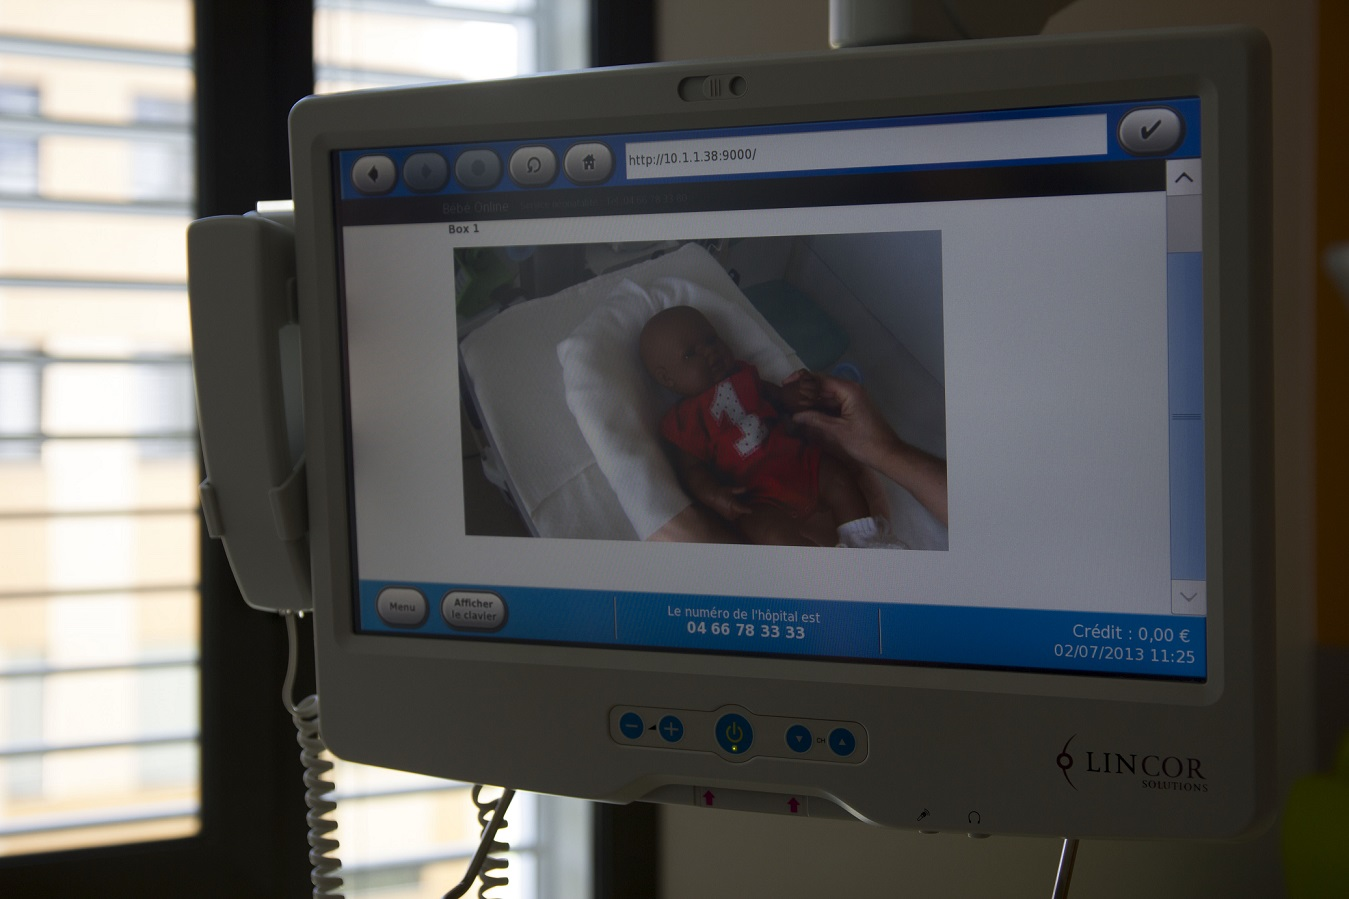
\includegraphics[width=5cm]{../images/bebeonline.jpg}	
				
\includegraphics[width=5cm]{../images/hammer_and_planks.jpg}	
				%\caption{A gauche : Formation du personnel médical aux outils déployés. A droite : Terminal avec BebeOnline}	
			\end{figure}
		\end{frame}	
		
		\begin{frame}{Hammer \& Planks}
			\begin{alertblock}{Un serious game pour la santé}
				• Un jeu vidéo sérieux d'aide à la réhabilitation motrice.\\
				• Adapté aux personnes hémiplégiques~: équilibre, membres supérieurs et tronc.\\
				• Jouable avec la la WiiBoard et la Kinect (main ou torse).
			\end{alertblock}
			\begin{exampleblock}{Un jeu vidéo ludique}
				• Existence d'une version grand public, au gameplay identique.\\
				• Plusieurs modes de jeu, différents ennemis et un univers riche et humoristique.
			\end{exampleblock}	
		\end{frame}
		
		\begin{frame}{TER : \emph{ZigFugl Meyer}}
			\begin{minipage}{0.40\linewidth}
				\begin{figure}
					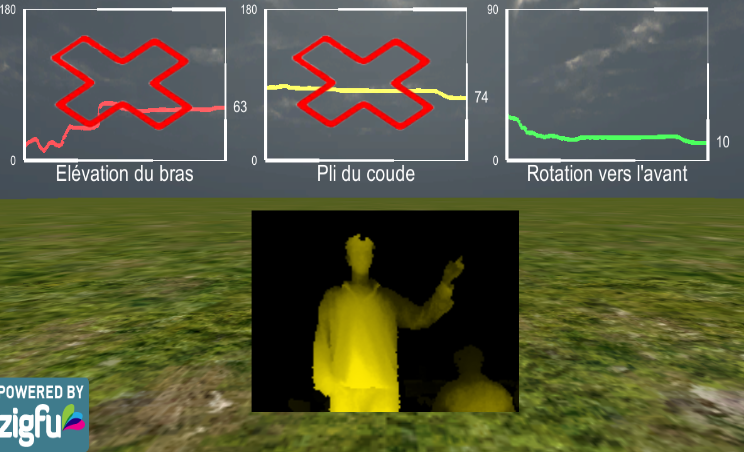
\includegraphics[width=4.2cm]{../images/zigfugl-meyer_1.png}\\
					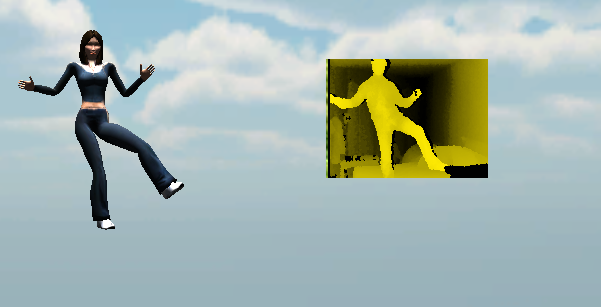
\includegraphics[width=4.2cm]{../images/zigfugl-meyer_2.png}
				\end{figure}
			\end{minipage}
			\begin{minipage}{6cm}%{0.55\linewidth}
				Idée : utiliser l'informatique pour l'évaluation de capacités motrices (Fugl Meyer assessment). 
					\begin{itemize}
						\item Utilisation de la Kinect comme interface naturelle.
						\item Expérimentation d'une gamification du test.
						\item Vérification automatique de la réussite de l'exercice.
					\end{itemize}
			\end{minipage}
		\end{frame}
	
	\section{Problématique et objectifs}
		\begin{frame}{Serious Games}
			\begin{block}{Qu'est-ce que c'est?}
				Application qui combine une intention sérieuse à des ressorts ludiques.
			\end{block}\pause
			\begin{exampleblock}{Utilisés dans :}
				Éducation, formation, entraînement, marketing, communication, santé.
			\end{exampleblock}	\pause
			\begin{alertblock}{Ne pas confondre}
				Serious game, serious gaming et apprentissage tangentiel
			\end{alertblock}
		\end{frame}
	
		\begin{frame}{Serious Games pour la rééducation}
			\begin{exampleblock}{Objectifs et qualités}
				• renforcer la motivation des patients.\\
				• oublier que c'est du travail. \\
				• augmenter le temps de travail.
			\end{exampleblock}\pause
			\begin{alertblock}{Un problème d'adaptation}
			Il est nécessaire de prendre en compte :\\
					• la pathologie et les capacités physiques du patient.\\
					• les objectifs et contraintes thérapeutiques.\\
					• son âge, son aisance avec les nouvelles technologies.\\
					• son niveau de joueur.
			\end{alertblock}
		\end{frame}
	
		\begin{frame}{Objectifs de stage}		
			\large{Comment proposer des jeux vidéo pour la santé adaptés?}
		\end{frame}
		
	\section{Proposition et réalisations}	
		\begin{frame}{Propositions}
		Adaptation des SG pour les personnes âgées et/ou hémiplégiques.
			\begin{block}{Approches}
				\begin{enumerate}
					\item Tests de H\&P.
					\item Recherche documentaire
					\item Enquête de terrain
				\end{enumerate}
			\end{block}\pause
			\begin{exampleblock}{Axes de travail}			
				\begin{enumerate}
					\item Ajuster les paramètres de H\&P via l'interface thérapeute.
					\item Proposition d'outils d'aide à la conception de jeux pour la santé.
					\item Suggestion d'une méthodologie de conception.
				\end{enumerate}
			\end{exampleblock}
		\end{frame}		
				
		\subsection{Ajustement des paramètres de H\&P}	
		\begin{frame}{Ajustement des paramètres de jeu}
				\begin{block}{Intérêts}
					• Contraindre le joueur à effectuer certains mouvements.\\
					• Varier le gameplay et donc maintenir la motivation.\\
					• Suivre l'évolution du joueur.
				\end{block}
			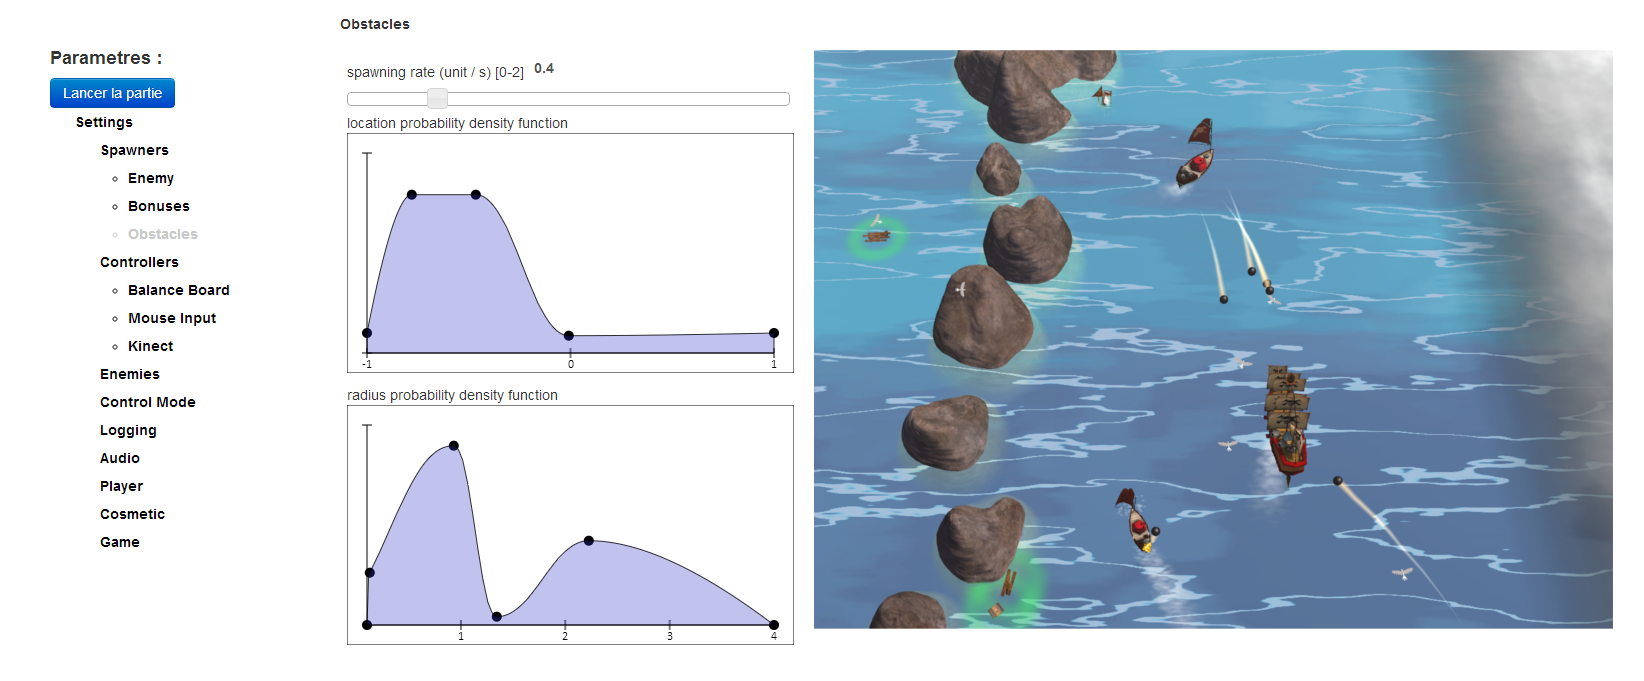
\includegraphics[width=10cm, height=4cm]{../images/comparatif_interface_rochers.png}
		\end{frame}			
			
		\begin{frame}{Interface thérapeutique}
		\setbeamercovered{transparent}
			\begin{block}{Quoi?}
				\begin{itemize}
					\item<1> Pouvoir réaliser plusieurs exercices de rééducation.
					\item<2> Ajuster le jeu durant une partie en fonction des besoins.
					\item<3> Proposer une expérience personnalisée à chaque joueur.
				\end{itemize}
			\end{block}
			\begin{block}{Comment?}
				\begin{itemize}
					\item<1> Définir et classer les objets paramétrables.
					\item<2> Avoir un accès direct aux paramètres ajustables.			
					\item<3> Créer et charger des configurations de valeurs.
				\end{itemize}
			\end{block}
			\setbeamercovered{invisible} 
		\end{frame}			
		
		\begin{frame}{Développement d'H\&P}
			\begin{block}{Travail initial}
				• Refactoring et extraction des paramètres.\\
				• Création de fichiers de 'vagues' pour le mode survie.\\
				• Correction de bugs et développement de fonctionnalités.
			\end{block}
			\begin{block}{Intégration des retours}
				• Système d'aspiration des bonus et de halo.\\
				• Ajustement de la GUI et des objets du jeu (taille, couleur)
			\end{block}
			\begin{figure}
				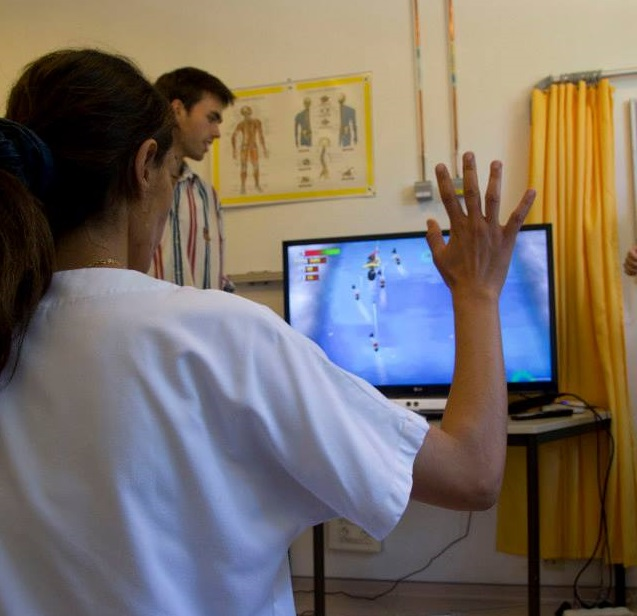
\includegraphics[width=5cm]{../images/test_lapeyronie_2.png}
			\end{figure}			
		\end{frame}
		
		\subsection{Outils d'aide à la conception}
		\begin{frame}{Aide à la conception de jeux pour la santé}
			\begin{exampleblock}{Faciliter le travail de conception}
			• Fournir des informations utiles ou nécessaires à la conception.\\
			• Avoir une vision globale des éléments en jeu.\\
			• Proposer des pistes et encourager la création.
			\end{exampleblock}\pause
			
			\begin{block}{Acquisition des connaissances préalables}
				• Analyse de l'existant.\\
				• Connaissances médicales et enjeux thérapeutiques.\\
				• Exploration des théories utiles aux SG.				
			\end{block}
		\end{frame}
	
		\begin{frame}{Productions : coté jeu}
			\begin{block}{Classification des types de jeux vidéo (par gameplay)}
				Informer des possibilités de gameplays classiques et fiables.\\
				Permet de faire un premier rapprochement entre l'enjeu sérieux et la dimension ludique.
			\end{block}\pause
			\begin{block}{Propositions de contrôles naturels}
			Passer par les mouvements pour faire le lien entre le jeu et les exercices de rééducation.\\
			Mettre en lumière les jeux adaptés à un contrôle naturel.\\
			Proposer les contrôles les plus adaptés.
			\end{block}			
		\end{frame}
		
		\begin{frame}{Productions : côté sérieux}
			\begin{block}{Connaissances médicales}
			Explication ou vulgarisation des objectifs thérapeutiques, des pathologies ou des mécanismes médicaux en jeu.\\
			Comprendre la réhabilitation et le quotidien des patients et des thérapeutes.
			\end{block}
		\end{frame}	
		
		\begin{frame}{Productions : côté sérieux}
			\begin{figure}
			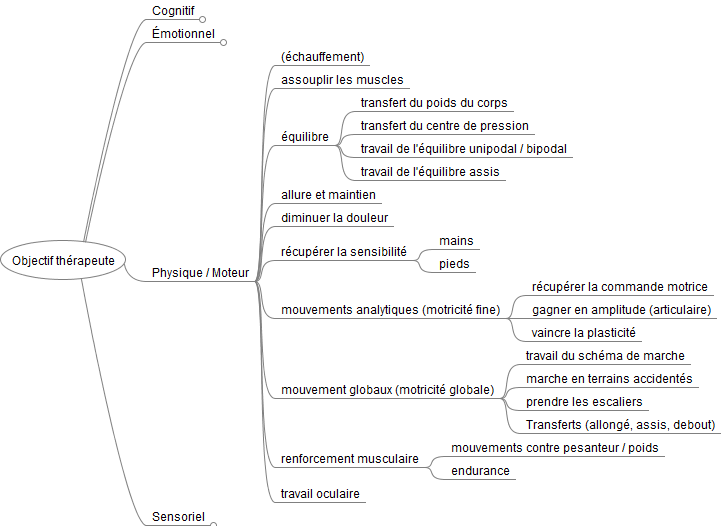
\includegraphics[width=10cm, height=6.5cm]{../images/objectifs_moteurs.png}
			\caption{Classement des objectifs thérapeutiques en rééducation}
			\end{figure}
		\end{frame}
			
		\subsection{Méthodologie de conception de SG}
		\begin{frame}{Méthodologie de conception}
			\begin{exampleblock}{Objectifs}
				• Concevoir des SG pour la santé.\\ \pause
				• Obtenir des jeux efficaces et qui seront joués.\\ \pause
				• Améliorer la conception : temps, qualité, réutilisabilité, satisfaction 
			\end{exampleblock} \pause
			\begin{alertblock}{Conception participative}
				• Intégrer au mieux les besoins des thérapeutes.\\
				• Intégrer l'expertise de différents domaines dès la phase de conception.\\
				• Se concentrer sur les objectifs et les impacts à réaliser.
			\end{alertblock}
		\end{frame}			
		
		\begin{frame}{Étapes de conception}
		\setbeamercovered{transparent}
			\begin{block}{Quoi?}
				\begin{enumerate}
					\item<1> Déterminer les objectifs : Pourquoi, Qui, Comment et Quoi? 
					\item<2> Comprendre les utilisateurs.
					\item<3> Imaginer les cas d'utilisation.
					\item<4> Illustrer et personnaliser l'utilisation de l'application.
				\end{enumerate}
			\end{block}
			\begin{block}{Comment?}
				\begin{enumerate}
					\item<1> Séance de conception participative.
					\item<2> Création d'une carte d'empathie.
					\item<3> Écriture des cas d'utilisation.
					\item<4> Création de storyboards.
				\end{enumerate}
			\end{block}
			\setbeamercovered{invisible}
		\end{frame}
		
		\begin{frame}{Application de la méthodologie}
			• conception lombalgie, verticalisation\\
			• poursuite du travail de TER : fugl meyer informatique
		\end{frame}
	
	\section{Perspectives}
		\begin{frame}
		 	- IT : Enregistrer ses propres config, ajouter de nouveaux jeux, proposer des sets de paramètres par objectif/exercices\\
			- publication de mes recherches : trouver où\\
			- poursuite du travail, amélioration des outils, enrichissement\\
			- évaluation et comparaison de la méthodologie\\
			- poursuite en travail de thèse : serious games, difficulté, cifre avec natkin
			- mission chez un kiné pour évaluation de jeu et game design.
		\end{frame}
	
	\section{Conclusion}
		\begin{frame}
			Travail sur un projet d'entreprise en équipe.
			Aspect R\&D, en solo puis en équipe pluridisciplinaire.
			Acquisition de beaucoup de connaissances, de contacts.
			trouver ce que je suis venu chercher en accord avec mes principes et souhaits
		\end{frame}

\end{document}